\documentclass[11pt,a4paper]{article}

\usepackage[margin=22mm,headheight=14pt]{geometry}

\usepackage{longtable,booktabs,array,hyperref,xcolor,tikz,fancyhdr}

\usepackage{fontspec,xeCJK}

\setmainfont[Ligatures=TeXOff]{Times New Roman}

\setsansfont[Ligatures=TeXOff]{Times New Roman}

\setmonofont[Ligatures=TeXOff,WordSpace={1,1,1}]{Times New Roman}

\setCJKmainfont{Noto Serif CJK SC}

\setCJKsansfont{Noto Serif CJK SC}

\setCJKmonofont{Noto Serif CJK SC}

\XeTeXgenerateactualtext=1

\definecolor{vulcan}{HTML}{BB3E23}

\pgfdeclarelayer{connections}\pgfdeclarelayer{edge labels}\pgfsetlayers{connections,main,edge labels}

\hypersetup{hidelinks}

\newcolumntype{L}[1]{>{\raggedright\arraybackslash}p{#1}}

\setlength{\emergencystretch}{3em}

\setlength{\parindent}{0pt}\setlength{\parskip}{5pt}

\pagestyle{fancy}\fancyhf{}\fancyhead[L]{\small\sffamily VULCAN}

\fancyhead[R]{\small Product design and verification}\fancyfoot[C]{\thepage}

\begin{document}

{\sffamily\huge\raggedright\textbf{Anvil-E1 Phase 2: Official Checkpoint-Slice Integration and Software-to-RTL Evaluation}\par}

{\large Technical Design and Verification Report}\par

15 October 2026 (\allowbreak{}UTC+\allowbreak{}8)\allowbreak{}\par\textcolor{vulcan}{\rule{\textwidth}{0.5pt}}

\begin{abstract}

Anvil-E1 is a modular,\allowbreak{} externally memory-backed SystemVerilog text-embedding engine implementing hybrid attention,\allowbreak{} per-layer embedding inputs,\allowbreak{} feedforward processing,\allowbreak{} masked mean pooling and Matryoshka prefix normalization. Phase 2 integrates authentic supplied Google EmbeddingGemma-2 BF16 checkpoint slices through deterministic signed-Q8.\allowbreak{}24 weight mapping and a zero-stage anvil\_\allowbreak{}e\_\allowbreak{}top wrapper.


All sixteen official-weight evaluations passed: 52 output words matched the independent integer oracle exactly,\allowbreak{} minimum FP32-to-RTL cosine similarity was 0.\allowbreak{}9999999998517652,\allowbreak{} and maximum absolute error was 1.\allowbreak{}2040138244628906e-5. Nine inherited configuration/\allowbreak{}seed runs,\allowbreak{} corruption sensitivity and reduced-configuration synthesis also passed. These measurements establish reduced mapped-slice execution,\allowbreak{} not full-checkpoint inference,\allowbreak{} upstream executable parity or physical performance.


\end{abstract}

\section{Architecture and design rationale}

Thirteen RTL files comprise twelve dedicated anvil\_\allowbreak{}e1 modules and the anvil\_\allowbreak{}e\_\allowbreak{}top integration wrapper. The wrapper contains exactly one parameter- and port-forwarding anvil\_\allowbreak{}e1\_\allowbreak{}top instance named core,\allowbreak{} adding no computation,\allowbreak{} storage or latency. A hardwired sequencer shares arithmetic and memory resources across transformer operations. Weights and sequence-sized intermediates remain external; on-chip storage is bounded by vector dimensions. Attention recomputes scores across three passes instead of retaining a sequence-squared score matrix,\allowbreak{} exchanging memory traffic and latency for bounded local storage. The forward equations are adopted parent-contract conventions,\allowbreak{} not independently demonstrated upstream executable behavior. [\allowbreak{}E001,\allowbreak{} E002,\allowbreak{} E015,\allowbreak{} E016]\allowbreak{}

\begin{center}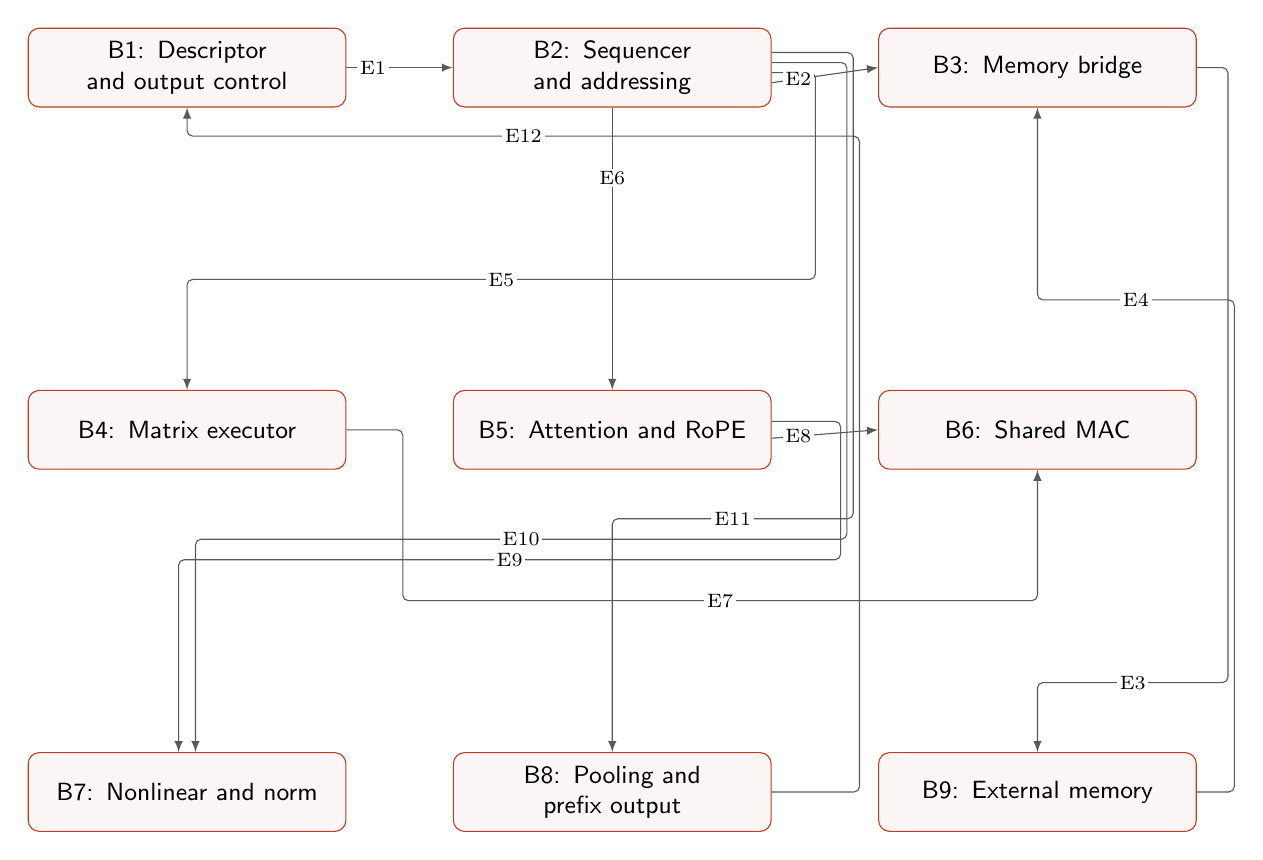
\begin{tikzpicture}[every node/.style={font=\small\sffamily},>=latex]

\node[draw=vulcan,rounded corners,fill=vulcan!4,text width=3.8cm,minimum height=1cm,align=center] (b0) at (0.0,0.0) {B1: Descriptor and output control};

\node[draw=vulcan,rounded corners,fill=vulcan!4,text width=3.8cm,minimum height=1cm,align=center] (b1) at (5.4,0.0) {B2: Sequencer and addressing};

\node[draw=vulcan,rounded corners,fill=vulcan!4,text width=3.8cm,minimum height=1cm,align=center] (b2) at (10.8,0.0) {B3: Memory bridge};

\node[draw=vulcan,rounded corners,fill=vulcan!4,text width=3.8cm,minimum height=1cm,align=center] (b3) at (0.0,-4.6) {B4: Matrix executor};

\node[draw=vulcan,rounded corners,fill=vulcan!4,text width=3.8cm,minimum height=1cm,align=center] (b4) at (5.4,-4.6) {B5: Attention and RoPE};

\node[draw=vulcan,rounded corners,fill=vulcan!4,text width=3.8cm,minimum height=1cm,align=center] (b5) at (10.8,-4.6) {B6: Shared MAC};

\node[draw=vulcan,rounded corners,fill=vulcan!4,text width=3.8cm,minimum height=1cm,align=center] (b6) at (0.0,-9.2) {B7: Nonlinear and norm};

\node[draw=vulcan,rounded corners,fill=vulcan!4,text width=3.8cm,minimum height=1cm,align=center] (b7) at (5.4,-9.2) {B8: Pooling and prefix output};

\node[draw=vulcan,rounded corners,fill=vulcan!4,text width=3.8cm,minimum height=1cm,align=center] (b8) at (10.8,-9.2) {B9: External memory};

\begin{pgfonlayer}{connections}

\draw[->,black!65] ([yshift=0.000cm]b0.east) -- coordinate[pos=0.25] (e0) ([yshift=0.000cm]b1.west);

\draw[->,black!65] ([yshift=-0.192cm]b1.east) -- coordinate[pos=0.25] (e1) ([yshift=0.000cm]b2.west);

\draw[->,black!65,rounded corners=2pt] ([yshift=0.000cm]b2.east) -- (13.220,0.000) -- (13.220,-7.810) -- coordinate[midway] (e2) (10.800,-7.810) -- ([xshift=0.000cm]b8.north);

\draw[->,black!65,rounded corners=2pt] ([yshift=0.000cm]b8.east) -- (13.300,-9.200) -- (13.300,-2.950) -- coordinate[midway] (e3) (10.800,-2.950) -- ([xshift=0.000cm]b2.south);

\draw[->,black!65,rounded corners=2pt] ([yshift=-0.064cm]b1.east) -- (7.980,-0.064) -- (7.980,-2.690) -- coordinate[midway] (e4) (0.000,-2.690) -- ([xshift=0.000cm]b3.north);

\draw[->,black!65] ([xshift=0.000cm]b1.south) -- coordinate[pos=0.25] (e5) ([xshift=0.000cm]b4.north);

\draw[->,black!65,rounded corners=2pt] ([yshift=0.000cm]b3.east) -- (2.740,-4.600) -- (2.740,-6.770) -- coordinate[midway] (e6) (10.800,-6.770) -- ([xshift=0.000cm]b5.south);

\draw[->,black!65] ([yshift=-0.107cm]b4.east) -- coordinate[pos=0.25] (e7) ([yshift=0.000cm]b5.west);

\draw[->,black!65,rounded corners=2pt] ([yshift=0.107cm]b4.east) -- (8.300,-4.493) -- (8.300,-6.250) -- coordinate[midway] (e8) (-0.107,-6.250) -- ([xshift=-0.107cm]b6.north);

\draw[->,black!65,rounded corners=2pt] ([yshift=0.064cm]b1.east) -- (8.380,0.064) -- (8.380,-5.990) -- coordinate[midway] (e9) (0.107,-5.990) -- ([xshift=0.107cm]b6.north);

\draw[->,black!65,rounded corners=2pt] ([yshift=0.192cm]b1.east) -- (8.460,0.192) -- (8.460,-5.730) -- coordinate[midway] (e10) (5.400,-5.730) -- ([xshift=0.000cm]b7.north);

\draw[->,black!65,rounded corners=2pt] ([yshift=0.000cm]b7.east) -- (8.540,-9.200) -- (8.540,-0.870) -- coordinate[midway] (e11) (0.000,-0.870) -- ([xshift=0.000cm]b0.south);

\end{pgfonlayer}

\begin{pgfonlayer}{edge labels}

\node[fill=white,inner sep=1pt,font=\scriptsize] at (e0) {E1};

\node[fill=white,inner sep=1pt,font=\scriptsize] at (e1) {E2};

\node[fill=white,inner sep=1pt,font=\scriptsize] at (e2) {E3};

\node[fill=white,inner sep=1pt,font=\scriptsize] at (e3) {E4};

\node[fill=white,inner sep=1pt,font=\scriptsize] at (e4) {E5};

\node[fill=white,inner sep=1pt,font=\scriptsize] at (e5) {E6};

\node[fill=white,inner sep=1pt,font=\scriptsize] at (e6) {E7};

\node[fill=white,inner sep=1pt,font=\scriptsize] at (e7) {E8};

\node[fill=white,inner sep=1pt,font=\scriptsize] at (e8) {E9};

\node[fill=white,inner sep=1pt,font=\scriptsize] at (e9) {E10};

\node[fill=white,inner sep=1pt,font=\scriptsize] at (e10) {E11};

\node[fill=white,inner sep=1pt,font=\scriptsize] at (e11) {E12};

\end{pgfonlayer}

\end{tikzpicture}\end{center}

{\small Functional block map, not a gate-level netlist. Edge identifiers match the directed relationships below. Crossings do not denote junctions; separate attachment points preserve arrow directions.}

{\small\begin{longtable}{@{}L{0.24\textwidth}L{0.7\textwidth}@{}}\toprule

\textbf{Block} & \textbf{Responsibility}\\\midrule\endhead

B1: Descriptor and output control & Latches descriptors,\allowbreak{} validates input arrays,\allowbreak{} controls job ownership,\allowbreak{} and registers embedding and completion outputs.\\[3pt]

B2: Sequencer and addressing & Schedules the forward path,\allowbreak{} calculates tensor and scratch addresses,\allowbreak{} and arbitrates shared-resource ownership.\\[3pt]

B3: Memory bridge & Registers requests and responses,\allowbreak{} permitting one outstanding external transaction,\allowbreak{} including acknowledged writes.\\[3pt]

B4: Matrix executor & Buffers an input vector,\allowbreak{} streams row-major weights and captures complete shared-MAC reductions.\\[3pt]

B5: Attention and RoPE & Executes grouped-query hybrid attention and split-half absolute-position rotations using shared arithmetic.\\[3pt]

B6: Shared MAC & Forms signed 64-bit products and complete 96-bit accumulations with operation-boundary rounding.\\[3pt]

B7: Nonlinear and norm & Provides iterative nonlinear functions,\allowbreak{} weighted RMS normalization and epsilon-free L2 normalization.\\[3pt]

B8: Pooling and prefix output & Accumulates valid-token projections,\allowbreak{} computes their mean and normalizes the requested leading channels.\\[3pt]

B9: External memory & Integrator-owned storage for packed weights,\allowbreak{} IDs,\allowbreak{} positions,\allowbreak{} masks and sequence-sized scratch.\\[3pt]

\bottomrule\end{longtable}}

{\small\begin{longtable}{@{}L{0.24\textwidth}L{0.7\textwidth}@{}}\toprule

\textbf{Directed relationship} & \textbf{Meaning}\\\midrule\endhead

E1: B1 to B2 & Validated job and execution ownership\\[3pt]

E2: B2 to B3 & Arbitrated memory commands\\[3pt]

E3: B3 to B9 & Registered read/\allowbreak{}write requests\\[3pt]

E4: B9 to B3 & Ordered data/\allowbreak{}error responses\\[3pt]

E5: B2 to B4 & Projection scheduling\\[3pt]

E6: B2 to B5 & Head,\allowbreak{} layer and position scheduling\\[3pt]

E7: B4 to B6 & Exclusive MAC operands and enables\\[3pt]

E8: B5 to B6 & Score and rotation products\\[3pt]

E9: B5 to B7 & Exponential and trigonometric operations\\[3pt]

E10: B2 to B7 & Normalization and nonlinear scheduling\\[3pt]

E11: B2 to B8 & Projected tokens,\allowbreak{} masks and prefix length\\[3pt]

E12: B8 to B1 & Embedding words and completion\\[3pt]

\bottomrule\end{longtable}}

\section{Interfaces and configuration}

{\small\begin{longtable}{@{}L{0.2\textwidth}L{0.12\textwidth}L{0.1\textwidth}L{0.48\textwidth}@{}}\toprule

\textbf{Signal /\allowbreak{} group} & \textbf{Direction} & \textbf{Width} & \textbf{Contract}\\\midrule\endhead

clk,\allowbreak{} rst\_\allowbreak{}n & Input & 1 bit each & Rising-edge clock and asynchronous active-low reset. Asserted reset zeros every public output and payload and cancels active work. The external fabric must share reset or flush obsolete responses.\\[3pt]

job\_\allowbreak{}valid,\allowbreak{} job\_\allowbreak{}ready; job\_\allowbreak{}tokens,\allowbreak{} job\_\allowbreak{}output\_\allowbreak{}dim & Input valid and descriptor; output ready & 1-bit handshake; 32-bit count; 16-bit dimension & Acceptance occurs on a rising edge with job\_\allowbreak{}valid and job\_\allowbreak{}ready asserted. Hold descriptor fields stable until that edge; the controller then latches them. Count is 1..MAX\_\allowbreak{}SEQ\_\allowbreak{}LEN; dimension selects E,\allowbreak{} 2E/\allowbreak{}3,\allowbreak{} E/\allowbreak{}3 or E/\allowbreak{}6. Further acceptance is disabled until completion retirement.\\[3pt]

weights\_\allowbreak{}base,\allowbreak{} tokens\_\allowbreak{}base,\allowbreak{} positions\_\allowbreak{}base,\allowbreak{} mask\_\allowbreak{}base,\allowbreak{} scratch\_\allowbreak{}base & Input & 64 bits each & Four-byte-aligned byte addresses,\allowbreak{} latched with the descriptor. Hold them stable until descriptor acceptance; they need not remain fixed afterward. The host guarantees nonoverlapping regions,\allowbreak{} keeps initialized weights,\allowbreak{} IDs,\allowbreak{} positions and masks unchanged until completion,\allowbreak{} and reserves scratch for DUT writes. Hardware rejects exclusive-end address overflow. Memory responses and handshake inputs remain active protocol signals,\allowbreak{} not immutable job data. [\allowbreak{}E006,\allowbreak{} E015,\allowbreak{} E016]\allowbreak{}\\[3pt]

mem\_\allowbreak{}req\_\allowbreak{}valid,\allowbreak{} mem\_\allowbreak{}req\_\allowbreak{}ready,\allowbreak{} mem\_\allowbreak{}req\_\allowbreak{}write,\allowbreak{} mem\_\allowbreak{}req\_\allowbreak{}addr,\allowbreak{} mem\_\allowbreak{}req\_\allowbreak{}wdata & Output request; input ready & 1-bit controls; 64-bit address; 32-bit data & Registered single-word requests remain stable through stalls. Acceptance requires valid and ready on a rising edge. At most one request is outstanding.\\[3pt]

mem\_\allowbreak{}rsp\_\allowbreak{}valid,\allowbreak{} mem\_\allowbreak{}rsp\_\allowbreak{}ready,\allowbreak{} mem\_\allowbreak{}rsp\_\allowbreak{}rdata,\allowbreak{} mem\_\allowbreak{}rsp\_\allowbreak{}error & Input response; output ready & 1-bit controls/\allowbreak{}error; 32-bit data & Service every accepted request,\allowbreak{} including writes,\allowbreak{} with one ordered response. Hold a valid response and its payload until acceptance. Response readiness follows request acceptance; there is no combinational zero-latency shortcut.\\[3pt]

emb\_\allowbreak{}valid,\allowbreak{} emb\_\allowbreak{}ready,\allowbreak{} emb\_\allowbreak{}data,\allowbreak{} emb\_\allowbreak{}index,\allowbreak{} emb\_\allowbreak{}last & Output stream; input ready & 1-bit handshake/\allowbreak{}last; signed 32-bit data; 16-bit index & Signed Q8.\allowbreak{}24 words use ascending zero-based indices. Data,\allowbreak{} index and last remain stable while stalled. A one-channel prefix emits index zero with last asserted. The recipient may vary emb\_\allowbreak{}ready according to its protocol needs.\\[3pt]

done\_\allowbreak{}valid,\allowbreak{} done\_\allowbreak{}ready,\allowbreak{} done\_\allowbreak{}error,\allowbreak{} busy & Output status; input completion ready & 1-bit handshake/\allowbreak{}busy; 4-bit error & Completion is separately registered and held until accepted. Errors are 0 success,\allowbreak{} 1 invalid descriptor,\allowbreak{} 2 invalid token/\allowbreak{}position/\allowbreak{}mask,\allowbreak{} 3 memory error,\allowbreak{} 4 all masked and 5 address overflow. Errors emit no successful embedding. Busy remains asserted and job\_\allowbreak{}ready low through output/\allowbreak{}completion stalls; completion acceptance permits return to idle.\\[3pt]

\bottomrule\end{longtable}}

{\small\begin{longtable}{@{}L{0.23\textwidth}L{0.12\textwidth}L{0.57\textwidth}@{}}\toprule

\textbf{Parameter} & \textbf{Default} & \textbf{Meaning /\allowbreak{} supported values}\\\midrule\endhead

VOCAB\_\allowbreak{}SIZE & 262144 & Positive; all token IDs must be below this value,\allowbreak{} including masked entries.\\[3pt]

HIDDEN\_\allowbreak{}SIZE,\allowbreak{} PER\_\allowbreak{}LAYER\_\allowbreak{}INPUT\_\allowbreak{}SIZE,\allowbreak{} INTERMEDIATE\_\allowbreak{}SIZE & 512,\allowbreak{} 512,\allowbreak{} 2048 & Each 1..65535. Per-layer input width is independently configurable.\\[3pt]

EMBEDDING\_\allowbreak{}DIM & 768 & 6..65535 and divisible by six; default output prefixes are 768,\allowbreak{} 512,\allowbreak{} 256 and 128.\\[3pt]

NUM\_\allowbreak{}LAYERS & 24 & 1..65535. Indices congruent to five modulo six use full attention: 5,\allowbreak{} 11,\allowbreak{} 17 and 23 at defaults.\\[3pt]

NUM\_\allowbreak{}Q\_\allowbreak{}HEADS,\allowbreak{} LOCAL\_\allowbreak{}KV\_\allowbreak{}HEADS,\allowbreak{} FULL\_\allowbreak{}KV\_\allowbreak{}HEADS & 4,\allowbreak{} 2,\allowbreak{} 1 & Positive; query-head count is at most 65535 and divisible by each KV-head count.\\[3pt]

LOCAL\_\allowbreak{}HEAD\_\allowbreak{}DIM,\allowbreak{} FULL\_\allowbreak{}HEAD\_\allowbreak{}DIM & 256,\allowbreak{} 512 & Positive even widths; each query-head-count times head-width product must not exceed 65535.\\[3pt]

SLIDING\_\allowbreak{}WINDOW,\allowbreak{} MAX\_\allowbreak{}SEQ\_\allowbreak{}LEN & 512,\allowbreak{} 262144 & Positive. Positions must be below MAX\_\allowbreak{}SEQ\_\allowbreak{}LEN; local attention requires absolute position distance strictly below SLIDING\_\allowbreak{}WINDOW.\\[3pt]

\bottomrule\end{longtable}}

\section{Behavior and corner cases}

\subsection{Official-weight mapping}

Of 55 supplied tensors,\allowbreak{} 39 text tensors provide inference coefficients. Official configuration A uses (\allowbreak{}V,\allowbreak{}H,\allowbreak{}P,\allowbreak{}I,\allowbreak{}E,\allowbreak{}L,\allowbreak{}Q,\allowbreak{}localKV,\allowbreak{}fullKV,\allowbreak{}localD,\allowbreak{}fullD,\allowbreak{}window,\allowbreak{}maxSeq)\allowbreak{}=\allowbreak{}(\allowbreak{}16,\allowbreak{}4,\allowbreak{}4,\allowbreak{}8,\allowbreak{}6,\allowbreak{}6,\allowbreak{}2,\allowbreak{}1,\allowbreak{}1,\allowbreak{}2,\allowbreak{}4,\allowbreak{}2,\allowbreak{}8)\allowbreak{}. Destination layers 0..4 repeat official layer 0; layer 5 uses official layer 5. Matrices select leading rows/\allowbreak{}columns using loaded source strides,\allowbreak{} not flattened prefixes. Global PLE selects rows 0..23 and columns 0..3,\allowbreak{} assigning four distinct rows per destination layer; layer 5 therefore uses available rows 20..23,\allowbreak{} not unavailable original layer-5 coordinates. Packing produces 107 destination tensors: five globals lexically,\allowbreak{} then ascending destination layer and lexical suffix,\allowbreak{} with row-major four-byte elements. No coefficients are fabricated,\allowbreak{} rescaled,\allowbreak{} neutralized or accuracy-selected. [\allowbreak{}E002,\allowbreak{} E031]\allowbreak{}

\subsection{Forward computation}

Token embeddings are multiplied by sqrt(\allowbreak{}H)\allowbreak{}. Global PLE projection is divided by sqrt(\allowbreak{}H)\allowbreak{},\allowbreak{} reshaped per layer and unit-offset RMS-normalized. Each layer performs input RMSNorm; q/\allowbreak{}k/\allowbreak{}v projections; per-head q/\allowbreak{}k RMSNorm; RoPE and attention; output projection,\allowbreak{} post-attention norm and residual; pre-feedforward norm,\allowbreak{} tanh-GELU(\allowbreak{}gate)\allowbreak{}*\allowbreak{}up,\allowbreak{} down projection,\allowbreak{} post-feedforward norm and residual; GELU-gated PLE multiplication,\allowbreak{} projection,\allowbreak{} post-PLE norm and residual; then layer\_\allowbreak{}scalar. Attention width remains Q*\allowbreak{}D until output projection. Final RMSNorm and embedding projection precede masked mean pooling,\allowbreak{} prefix selection and selected-prefix L2 normalization. Projections are bias-free and inference dropout is zero. [\allowbreak{}E001]\allowbreak{}

\subsection{Attention and masks}

Attention is bidirectional with contiguous grouped-query mapping. Local/\allowbreak{}full RoPE bases are 10000/\allowbreak{}1000000; rotations pair split halves at supplied absolute positions. Local keys require abs(\allowbreak{}key\_\allowbreak{}position-query\_\allowbreak{}position)\allowbreak{}<window; full layers see all valid keys. Explicit masks select keys and pooling contributions. There is no automatic token insertion,\allowbreak{} PAD inference or prompt exclusion. All-masked jobs fail; a nonempty zero pooled vector succeeds with zero output. [\allowbreak{}E001]\allowbreak{}

\subsection{Numerical contract and correction}

External weights,\allowbreak{} activations and outputs are signed Q8.\allowbreak{}24,\allowbreak{} rounded nearest/\allowbreak{}ties-even and saturated to [\allowbreak{}-128,\allowbreak{}128-2\textasciicircum{}-24]\allowbreak{}. Products are signed 64-bit and complete reductions retain at least 96 bits. Weighted RMSNorm computes x/\allowbreak{}sqrt(\allowbreak{}mean(\allowbreak{}x²)\allowbreak{}+\allowbreak{}epsilon)\allowbreak{}*\allowbreak{}(\allowbreak{}1+\allowbreak{}w)\allowbreak{},\allowbreak{} adding EPSILON\_\allowbreak{}Q48=\allowbreak{}281474977 after ties-even rounding of the complete Q48 mean-square reduction. The earlier Q8.\allowbreak{}24-first epsilon,\allowbreak{} 17/\allowbreak{}2\textasciicircum{}24,\allowbreak{} caused official FP32 error-gate failures despite exact integer agreement. Direct Q48 epsilon representation resolves that denominator-precision defect without a legacy mode. L2 remains epsilon-free; nonfinite text coefficients are rejected. [\allowbreak{}E002,\allowbreak{} E011,\allowbreak{} E063]\allowbreak{}

\subsection{Nonlinear and cycle boundaries}

Nonlinear series use Q40 internal arithmetic. Exp uses an 18-term recurrence; sin/\allowbreak{}cos use range reduction and iterative series; GELU uses the tanh approximation and asymptotic handling at |x|>=\allowbreak{}8. Attention skips softmax differences below -16. RMS normalization retains a high-precision denominator and an 80-step integer square root. Memory-command capture,\allowbreak{} public request acceptance,\allowbreak{} response capture and consumer retirement are distinct boundaries. Embedding and completion holding stages cannot be bypassed; the wrapper adds zero stages. [\allowbreak{}E001]\allowbreak{}

\section{Verification methods and measured results}

\subsection{Authoritative defaults,\allowbreak{} interfaces and packing}

\textbf{Method.} Retained architecture checks examined both tops,\allowbreak{} default elaboration,\allowbreak{} address boundaries,\allowbreak{} the complete packing contract,\allowbreak{} illegal geometry and BF16 conversion/\allowbreak{}rejection.

\textbf{Result.} Passed: 413 expanded tensors,\allowbreak{} full layers 5/\allowbreak{}11/\allowbreak{}17/\allowbreak{}23,\allowbreak{} 65280 finite BF16 encodings checked,\allowbreak{} 256 nonfinite encodings rejected and seven illegal-parameter cases diagnosed. The retained architecture result was not rerun during execution-budget recovery.

{\small Evidence: E052,\allowbreak{} E003,\allowbreak{} E016,\allowbreak{} E026,\allowbreak{} E033}

\subsection{Authentic supplied-weight consistency}

\textbf{Method.} Streamed file SHA-256; parsed raw BF16 safetensors; validated tensor shapes,\allowbreak{} extents,\allowbreak{} ranges and hashes; independently checked supplied FP32/\allowbreak{}Q8.\allowbreak{}24 coordinates.

\textbf{Result.} All 55 tensor payloads passed,\allowbreak{} including excluded vision payloads; 39 text tensors supplied execution and 11266 JSON coordinates were checked. Safetensors SHA-256 is 3a310d77\allowbreak{}33a28f53\allowbreak{}3b611eb7\allowbreak{}525f5973\allowbreak{}03980c2a\allowbreak{}b2f89048\allowbreak{}7a9a1fcb\allowbreak{}f0366bfb. Mapped-image SHA-256 is 2cf8db51\allowbreak{}0462a099\allowbreak{}90f2d66c\allowbreak{}34598486\allowbreak{}6d0d6374\allowbreak{}d6997b7f\allowbreak{}a4c203a9\allowbreak{}e5e1e147.

{\small Evidence: E031,\allowbreak{} E063}

\subsection{Official FP32 software versus actual RTL}

\textbf{Method.} Icarus compiled actual RTL with -g2012; vvp executed four sequences at dimensions 6/\allowbreak{}4/\allowbreak{}2/\allowbreak{}1. Software decoded raw BF16 to FP32 using struct,\allowbreak{} documented rounding boundaries and mathematical nonlinearities,\allowbreak{} independently of the integer oracle.

\textbf{Result.} All 16 jobs and 52 words passed with zero integer mismatches. Minimum cosine was 0.\allowbreak{}9999999998517652 against 0.\allowbreak{}999; maximum absolute error was 1.\allowbreak{}2040138244628906e-5 against 0.\allowbreak{}002. Worst per-job MAE was 6.\allowbreak{}884336471557617e-6 and RMSE 8.\allowbreak{}600952306391626e-6. Maximum absolute software/\allowbreak{}RTL norm difference was 7.\allowbreak{}76098445509632e-8 against 0.\allowbreak{}002. Official weight conversion and integer operations recorded zero saturations.

{\small Evidence: E063,\allowbreak{} E031,\allowbreak{} E032,\allowbreak{} E039}

\subsection{Measured cycle-based throughput}

\textbf{Method.} Parsed accepted public descriptor,\allowbreak{} embedding and completion edges,\allowbreak{} including stalls. Latency equals destination-edge number minus descriptor-edge number,\allowbreak{} not an inclusive edge count.

\textbf{Result.} For dimensions 6/\allowbreak{}4/\allowbreak{}2/\allowbreak{}1,\allowbreak{} completion cycles were [\allowbreak{}22654,\allowbreak{}22625,\allowbreak{}22620,\allowbreak{}22613]\allowbreak{} for [\allowbreak{}2]\allowbreak{}; [\allowbreak{}48400,\allowbreak{}48383,\allowbreak{}48365,\allowbreak{}48374]\allowbreak{} for [\allowbreak{}2,\allowbreak{}3]\allowbreak{}; [\allowbreak{}70669,\allowbreak{}70665,\allowbreak{}70643,\allowbreak{}70637]\allowbreak{} for [\allowbreak{}2,\allowbreak{}4,\allowbreak{}7]\allowbreak{}; and [\allowbreak{}220274,\allowbreak{}220247,\allowbreak{}220239,\allowbreak{}220232]\allowbreak{} for [\allowbreak{}2,\allowbreak{}3,\allowbreak{}4,\allowbreak{}5,\allowbreak{}6,\allowbreak{}7,\allowbreak{}8,\allowbreak{}1]\allowbreak{}. Cycles/\allowbreak{}submitted-token ranged 22613..27534.\allowbreak{}25; tokens/\allowbreak{}cycle ranged 3.\allowbreak{}6318403443e-5..4.\allowbreak{}4222349976e-5. The comparison ledger separately records first/\allowbreak{}last embedding edges,\allowbreak{} valid-token denominators and jobs/\allowbreak{}cycle.

{\small Evidence: E063,\allowbreak{} E031}

\subsection{Preserved functional and primitive behavior}

\textbf{Method.} Executed A/\allowbreak{}B/\allowbreak{}C at seeds 17/\allowbreak{}89/\allowbreak{}203 with exact scoreboards,\allowbreak{} independent quantized-input mathematical comparisons,\allowbreak{} fault/\allowbreak{}reset traffic,\allowbreak{} protocol coverage and primitive/\allowbreak{}norm gates.

\textbf{Result.} All nine inherited runs passed,\allowbreak{} covering full-layer indices 5/\allowbreak{}11/\allowbreak{}17/\allowbreak{}23. GELU,\allowbreak{} exp and sin/\allowbreak{}cos satisfied absolute-error limits 2e-4,\allowbreak{} 2e-6 and 2e-5; representable nonzero reciprocal/\allowbreak{}rsqrt results satisfied relative error 2e-4. Directed small/\allowbreak{}zero denominators distinguished Q48 epsilon from the historical constant and preserved zero-vector L2 behavior.

{\small Evidence: E063,\allowbreak{} E027,\allowbreak{} E029,\allowbreak{} E034}

\subsection{Scoreboard corruption sensitivity}

\textbf{Method.} Freshly compiled and executed a successful official job,\allowbreak{} validated its original trace,\allowbreak{} changed exactly one accepted embedding word by one Q8.\allowbreak{}24 LSB in a private copy,\allowbreak{} and reapplied the identical scoreboard.

\textbf{Result.} The original trace passed. Changing job 0/\allowbreak{}index 0 from 11924784 to 11924785 produced the specific expected/\allowbreak{}observed exact-data mismatch. The altered trace is negative-control evidence only. The inherited functional negative control also passed.

{\small Evidence: E064,\allowbreak{} E063,\allowbreak{} E027}

\subsection{Synthesizable connected implementation}

\textbf{Method.} Yosys synthesized A and B under anvil\_\allowbreak{}e\_\allowbreak{}top using hierarchy checking,\allowbreak{} proc,\allowbreak{} opt,\allowbreak{} memory,\allowbreak{} check -assert,\allowbreak{} statistics and retained JSON netlists.

\textbf{Result.} Both passed wrapper-forwarding,\allowbreak{} required-descendant,\allowbreak{} connectivity,\allowbreak{} no-latch and no-unresolved/\allowbreak{}blackbox checks. Structural traversal counted 237 sequential/\allowbreak{}235 arithmetic cells for A and 319/\allowbreak{}247 for B. These generic structural counts are not technology area or timing measurements.

{\small Evidence: E065,\allowbreak{} E038}

\section{Integration and use}

Instantiate anvil\_\allowbreak{}e\_\allowbreak{}top and compile all rtl/\allowbreak{}*\allowbreak{}.sv; direct anvil\_\allowbreak{}e1\_\allowbreak{}top compatibility remains. Delivered checks require Python 3 standard library,\allowbreak{} iverilog,\allowbreak{} vvp and Yosys; NumPy is unnecessary.


Initialize packed weights and separate little-endian 32-bit ID,\allowbreak{} position and mask arrays. Reserve scratch bytes 4*\allowbreak{}N*\allowbreak{}(\allowbreak{}2*\allowbreak{}H+\allowbreak{}L*\allowbreak{}P+\allowbreak{}(\allowbreak{}Q+\allowbreak{}2*\allowbreak{}max(\allowbreak{}localKV,\allowbreak{}fullKV)\allowbreak{})\allowbreak{}*\allowbreak{}max(\allowbreak{}localD,\allowbreak{}fullD)\allowbreak{})\allowbreak{}. Scratch stores current/\allowbreak{}next hidden states,\allowbreak{} PLE and Q/\allowbreak{}K/\allowbreak{}V; do not preload hidden states or expected outputs.


Use design/\allowbreak{}pack\_\allowbreak{}model.\allowbreak{}py only with a complete authoritative default checkpoint: \texttt{python3 design/\allowbreak{}pack\_\allowbreak{}model.\allowbreak{}py --input model.\allowbreak{}safetensors --output weights.\allowbreak{}q24.\allowbreak{}bin --inventory weights.\allowbreak{}inventory.\allowbreak{}json}. Output parent directories must exist. The supplied partial official file is deliberately rejected; tests/\allowbreak{}official.\allowbreak{}py constructs the separate reduced evaluation image.


Assert reset with the memory fabric reset or flushed. Hold job\_\allowbreak{}tokens,\allowbreak{} job\_\allowbreak{}output\_\allowbreak{}dim and all five base addresses stable until the job\_\allowbreak{}valid\&\&job\_\allowbreak{}ready accepting edge; the controller latches the descriptor. Keep initialized weights,\allowbreak{} IDs,\allowbreak{} positions and masks unchanged until completion,\allowbreak{} and reserve scratch for DUT writes. During execution,\allowbreak{} actively service ordered memory responses and output/\allowbreak{}completion ready/\allowbreak{}valid handshakes; these signals are not frozen. Consume embedding transfers,\allowbreak{} inspect done\_\allowbreak{}error and retire completion through done\_\allowbreak{}valid\&\&done\_\allowbreak{}ready. [\allowbreak{}E006,\allowbreak{} E015,\allowbreak{} E016]\allowbreak{}


The recorded functional invocation is \texttt{python3 tests/\allowbreak{}verify.\allowbreak{}py --check functional --output evidence/\allowbreak{}verification/\allowbreak{}functional --timeout-s 230 --configs A,\allowbreak{}B,\allowbreak{}C --seeds 17,\allowbreak{}89,\allowbreak{}203 --repair-of evidence/\allowbreak{}verification/\allowbreak{}functional/\allowbreak{}attempt-20261015T082929570124Z/\allowbreak{}receipt.\allowbreak{}json}. Complete vectors,\allowbreak{} metrics,\allowbreak{} identities and cycle measurements are in evidence/\allowbreak{}verification/\allowbreak{}functional/\allowbreak{}official\_\allowbreak{}weights\_\allowbreak{}comparison.\allowbreak{}json; inherited results are in the producing attempt's run-ledger.\allowbreak{}json.


\section{Limitations and acceptance boundary}

Official execution is a deterministic reduced slice with repeated layer-0 coefficients,\allowbreak{} not original-geometry complete-checkpoint inference. In the stated geometry order,\allowbreak{} B=\allowbreak{}(\allowbreak{}20,\allowbreak{}6,\allowbreak{}4,\allowbreak{}10,\allowbreak{}12,\allowbreak{}12,\allowbreak{}4,\allowbreak{}2,\allowbreak{}1,\allowbreak{}2,\allowbreak{}4,\allowbreak{}3,\allowbreak{}8)\allowbreak{} and C=\allowbreak{}(\allowbreak{}16,\allowbreak{}4,\allowbreak{}4,\allowbreak{}8,\allowbreak{}6,\allowbreak{}24,\allowbreak{}4,\allowbreak{}2,\allowbreak{}1,\allowbreak{}2,\allowbreak{}4,\allowbreak{}2,\allowbreak{}4)\allowbreak{} extend inherited geometry coverage,\allowbreak{} not official-weight coverage.


Official cases use positions/\allowbreak{}masks [\allowbreak{}7]\allowbreak{}/\allowbreak{}[\allowbreak{}1]\allowbreak{},\allowbreak{} [\allowbreak{}1,\allowbreak{}2]\allowbreak{}/\allowbreak{}[\allowbreak{}1,\allowbreak{}1]\allowbreak{},\allowbreak{} [\allowbreak{}1,\allowbreak{}3,\allowbreak{}4]\allowbreak{}/\allowbreak{}[\allowbreak{}1,\allowbreak{}0,\allowbreak{}1]\allowbreak{},\allowbreak{} and positions 0..7 with six valid then two masked tokens. Accuracy applies to these cases,\allowbreak{} not arbitrary language workloads or embedding-retrieval quality.


Sixteen vision tensors are excluded: embed\_\allowbreak{}vision.\allowbreak{}embedding\_\allowbreak{}projection.\allowbreak{}weight; vision\_\allowbreak{}tower.\allowbreak{}patch\_\allowbreak{}embedder.\allowbreak{}input\_\allowbreak{}proj.\allowbreak{}weight and position\_\allowbreak{}embedding\_\allowbreak{}table; and vision\_\allowbreak{}tower.\allowbreak{}encoder.\allowbreak{}layers.\allowbreak{}0 suffixes input\_\allowbreak{}layernorm.\allowbreak{}weight,\allowbreak{} mlp.\allowbreak{}down\_\allowbreak{}proj.\allowbreak{}linear.\allowbreak{}weight,\allowbreak{} mlp.\allowbreak{}gate\_\allowbreak{}proj.\allowbreak{}linear.\allowbreak{}weight,\allowbreak{} mlp.\allowbreak{}up\_\allowbreak{}proj.\allowbreak{}linear.\allowbreak{}weight,\allowbreak{} post\_\allowbreak{}attention\_\allowbreak{}layernorm.\allowbreak{}weight,\allowbreak{} post\_\allowbreak{}feedforward\_\allowbreak{}layernorm.\allowbreak{}weight,\allowbreak{} pre\_\allowbreak{}feedforward\_\allowbreak{}layernorm.\allowbreak{}weight,\allowbreak{} self\_\allowbreak{}attn.\allowbreak{}k\_\allowbreak{}norm.\allowbreak{}weight,\allowbreak{} self\_\allowbreak{}attn.\allowbreak{}k\_\allowbreak{}proj.\allowbreak{}linear.\allowbreak{}weight,\allowbreak{} self\_\allowbreak{}attn.\allowbreak{}o\_\allowbreak{}proj.\allowbreak{}linear.\allowbreak{}weight,\allowbreak{} self\_\allowbreak{}attn.\allowbreak{}q\_\allowbreak{}norm.\allowbreak{}weight,\allowbreak{} self\_\allowbreak{}attn.\allowbreak{}q\_\allowbreak{}proj.\allowbreak{}linear.\allowbreak{}weight and self\_\allowbreak{}attn.\allowbreak{}v\_\allowbreak{}proj.\allowbreak{}linear.\allowbreak{}weight. Audio is also excluded.


Provenance establishes local consistency with supplied manifests,\allowbreak{} not independent remote retrieval. The floating path uses BF16 source coefficients with FP32 arithmetic; it does not establish BF16-activation execution or upstream executable parity.


The 10 ns testbench period is a simulation convention only. No physical clock rate,\allowbreak{} tokens/\allowbreak{}second capability,\allowbreak{} timing closure,\allowbreak{} power,\allowbreak{} technology area or default-size synthesis is established. Portable clean-directory reproduction and formal verification were not demonstrated.


\appendix\section{Source inventory}

Production inventory: 13 Verilog/\allowbreak{}SystemVerilog files; 2510 nonblank,\allowbreak{} non-comment lines. Source size is not a correctness or quality metric.

{\small\begin{longtable}{@{}L{0.61\textwidth}L{0.15\textwidth}L{0.15\textwidth}@{}}\toprule

\textbf{Production file} & \textbf{Physical lines} & \textbf{Code lines}\\\midrule\endhead

rtl/\allowbreak{}anvil\_\allowbreak{}e1\_\allowbreak{}address.\allowbreak{}sv & 173 & 164\\[3pt]

rtl/\allowbreak{}anvil\_\allowbreak{}e1\_\allowbreak{}attention.\allowbreak{}sv & 281 & 278\\[3pt]

rtl/\allowbreak{}anvil\_\allowbreak{}e1\_\allowbreak{}controller.\allowbreak{}sv & 179 & 175\\[3pt]

rtl/\allowbreak{}anvil\_\allowbreak{}e1\_\allowbreak{}mac.\allowbreak{}sv & 34 & 34\\[3pt]

rtl/\allowbreak{}anvil\_\allowbreak{}e1\_\allowbreak{}matvec.\allowbreak{}sv & 99 & 99\\[3pt]

rtl/\allowbreak{}anvil\_\allowbreak{}e1\_\allowbreak{}memory.\allowbreak{}sv & 65 & 65\\[3pt]

rtl/\allowbreak{}anvil\_\allowbreak{}e1\_\allowbreak{}nonlinear.\allowbreak{}sv & 243 & 237\\[3pt]

rtl/\allowbreak{}anvil\_\allowbreak{}e1\_\allowbreak{}norm.\allowbreak{}sv & 178 & 176\\[3pt]

rtl/\allowbreak{}anvil\_\allowbreak{}e1\_\allowbreak{}pool.\allowbreak{}sv & 162 & 161\\[3pt]

rtl/\allowbreak{}anvil\_\allowbreak{}e1\_\allowbreak{}rope.\allowbreak{}sv & 130 & 130\\[3pt]

rtl/\allowbreak{}anvil\_\allowbreak{}e1\_\allowbreak{}sequencer.\allowbreak{}sv & 778 & 762\\[3pt]

rtl/\allowbreak{}anvil\_\allowbreak{}e1\_\allowbreak{}top.\allowbreak{}sv & 158 & 158\\[3pt]

rtl/\allowbreak{}anvil\_\allowbreak{}e\_\allowbreak{}top.\allowbreak{}sv & 71 & 71\\[3pt]

\bottomrule\end{longtable}}

\section{Verification record index}

{\small\begin{longtable}{@{}L{0.57\textwidth}L{0.16\textwidth}L{0.17\textwidth}@{}}\toprule

\textbf{Recorded check} & \textbf{Outcome} & \textbf{Execution time (\allowbreak{}s)\allowbreak{}}\\\midrule\endhead

functional & passed & 225.\allowbreak{}508\\[3pt]

sensitivity & passed & 3.\allowbreak{}877\\[3pt]

synthesis & passed & 94.\allowbreak{}387\\[3pt]

\bottomrule\end{longtable}}

Execution times include tool and provider waiting; they are not hardware latency or model utilization.

{\small\begin{longtable}{@{}L{0.12\textwidth}L{0.82\textwidth}@{}}\toprule

\textbf{Reference} & \textbf{Original project-relative record}\\\midrule\endhead

E003 & design/\allowbreak{}pack\_\allowbreak{}model.\allowbreak{}py\\[3pt]

E016 & rtl/\allowbreak{}anvil\_\allowbreak{}e\_\allowbreak{}top.\allowbreak{}sv\\[3pt]

E026 & tests/\allowbreak{}architecture.\allowbreak{}py\\[3pt]

E027 & tests/\allowbreak{}behavior.\allowbreak{}py\\[3pt]

E029 & tests/\allowbreak{}model.\allowbreak{}py\\[3pt]

E031 & tests/\allowbreak{}official.\allowbreak{}py\\[3pt]

E032 & tests/\allowbreak{}official\_\allowbreak{}fp32.\allowbreak{}py\\[3pt]

E033 & tests/\allowbreak{}packing.\allowbreak{}py\\[3pt]

E034 & tests/\allowbreak{}primitives.\allowbreak{}py\\[3pt]

E038 & tests/\allowbreak{}synthesis.\allowbreak{}py\\[3pt]

E039 & tests/\allowbreak{}verify.\allowbreak{}py\\[3pt]

E052 & .vulcan/\allowbreak{}engineering/\allowbreak{}run-0002/\allowbreak{}attempt-0003/\allowbreak{}stdout.\allowbreak{}log\\[3pt]

E063 & .vulcan/\allowbreak{}engineering/\allowbreak{}run-0003/\allowbreak{}attempt-0003/\allowbreak{}stdout.\allowbreak{}log\\[3pt]

E064 & .vulcan/\allowbreak{}engineering/\allowbreak{}run-0003/\allowbreak{}attempt-0004/\allowbreak{}stdout.\allowbreak{}log\\[3pt]

E065 & .vulcan/\allowbreak{}engineering/\allowbreak{}run-0003/\allowbreak{}attempt-0005/\allowbreak{}stdout.\allowbreak{}log\\[3pt]

\bottomrule\end{longtable}}

\section{Document provenance}

Engineering was independently accepted for the recorded source and evidence identity. This is not exhaustive proof, hardware deployment or physical signoff. The companion REPORT.md records the exact report approval and source manifest, and links the English/Chinese journeys containing original failures and interventions. A report number identifies a generation attempt, not a new hardware revision.

No developer attribution was supplied; none has been inferred.

\end{document}
